\chapter{ARM Cortex-R functional safety additions over ARM Cortex-M}
\label{cortex_r_additions}

\section{ARM Cortex-R introduction}

The ARM Cortex-R is a family of 32-bit RISC processors. The cores are optimized for hard real-time and safety-critical applications. Cortex-R family consists of ARM Cortex-R4(F), ARM Cortex-R5(F), ARM Cortex-R7(F), ARM Cortex-R8(F and ARM Cortex-R52(F).

The Cortex-R is suitable for use in computer-controlled systems where very low latency and/or a high level of safety is required. An example of a hard real-time, safety-critical application would be a modern electronic braking system in an automobile. The system not only needs to be fast and responsive to a plethora of sensor data input but is also responsible for human safety. A failure of such a system could lead to severe injury or loss of life. Other examples of hard real-time and safety-critical applications include medical devices, electronic control units (ECU), robotics, etc.

\section{ARM Cortex-M introduction}

The ARM Cortex-M is also a family of 32-bit RISC processors. The cores are optimized for low-cost and energy-efficient microcontrollers. These cores are being used in tens of billions of consumer devices. The processors are intended for deeply embedded applications that require fast interrupt response features \citep{cortex_m4_reference}. The family consists of Cortex-M0, Cortex-M0+, Cortex-M1, Cortex-M3, Cortex-M4, Cortex-M7, Cortex-M23, Cortex-M33, Cortex-M35P and Cortex-M55.


\section{ARM Cortex-R processor lockstep}

\subsection{Dual core lockstep}

A Cortex-R5 processor group has four configurations, as described in \citep{cortex_r5_reference_manual}:
\begin{itemize}

    \item single CPU,
    \item twin CPU,
    \item redundant CPU and
    \item split/lock configuration.
    
\end{itemize}

Twin CPU configuration includes two individual and decoupled CPUs. Each CPU has its own
cache RAMs, debug logic and bus interfaces to the rest of the SoC. It
offers higher performance than a standard single CPU configuration. 

In redundant CPU configuration (lockstep), there is a functional CPU and a second redundant copy of the majority of the CPU logic. The redundant logic is driven by the same inputs as the functional logic.  In particular, the redundant CPU logic shares the same cache RAMs as the functional CPU. Therefore only one set of cache RAMs is required. The redundant logic
operates in lock-step with the CPU but does not directly affect the processor behavior in any way \citep{cortex_r5_reference_manual}. The CPU outputs to the cache RAMs are driven \textbf{exclusively} by the functional CPU. The comparison logic for comparing the outputs of the redundant logic and the functional logic can detect a single fault that occurs in either set of logic. ARM provides example comparison logic, but the developer can change it during the implementation. 

Split/lock configuration is a combination of two previously mentioned configurations. This mode includes two processors. If a processor is in split mode the CPUs work in twin CPU configuration, and if the processor is in lock mode it is in a redundant configuration.

\begin{figure}[H]

      \centering
      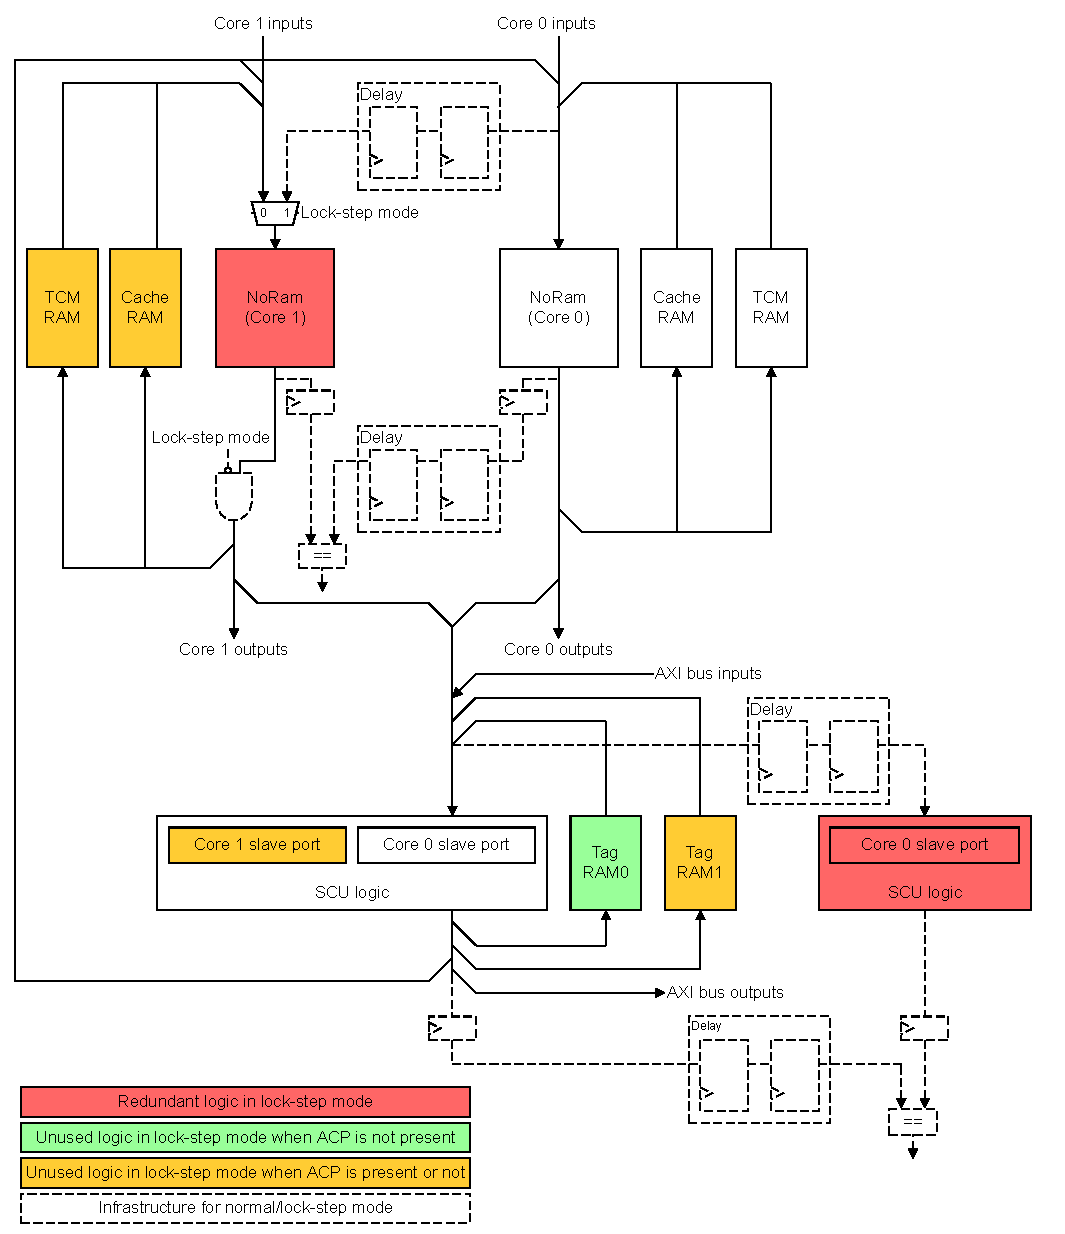
\includegraphics[width=1\linewidth]{images/split_lock_configuration.pdf}
      \caption{Split/lock configuration \citep{cortex_r8_reference_manual}}
      \label{fig:split_lock_configuration}
    
\end{figure}

\subsection{Triple core lockstep}

ARM triple-core lockstep architecture (TCLS) builds upon the industry success of the ARM Cortex-R5 dual-core lock-step (DCLS). The TCLS architecture adds a third redundant CPU unit to the DCLS Cortex-R5 system to achieve fail functional capabilities and hence increase the availability of the system \citep{TCLS_cortex_r}.

Cores in triple lockstep have shared data and instruction cache, but each Cortex-R5 has its own clock tree. \autoref{fig:tcls_architecture} shows the system level solution to mitigate soft errors occurring in the redundant CPUs. On the right side of the figure, the TCLS assist unit is visualized. TCLS assist unit supports the lockstep functioning of the CPUs and handles the error recovery process. The unit consists of a majority voter, error detection logic and synchronization logic.


\begin{figure}[H]

      \centering
      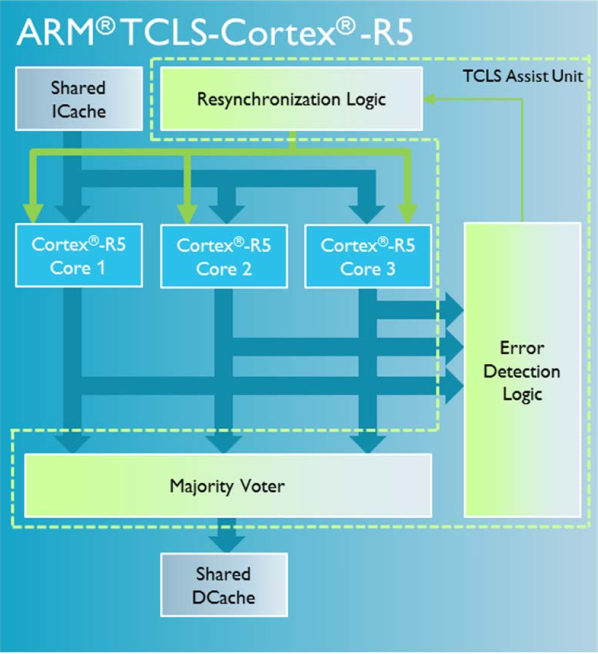
\includegraphics[width=0.7\linewidth]{images/tcls_architecture.png}
      \caption{ARM triple core lockstep of Cortex-R5 \citep{TCLS_cortex_r}}
      \label{fig:tcls_architecture}
    
\end{figure}

At every clock cycle, the instructions to execute are read
from the shared instruction cache or TCM (tightly coupled memory) and distributed to
the triplicated CPUs. The outputs from the CPUs are majority voted and
forwarded to the shared data cache, TCM, and I/O ports.
Simultaneously, the Error Detection logic checks if there is any
mismatch in the outputs delivered by the three CPUs. If there is
a mismatch, all CPUs are interrupted and the Error Detection
logic identifies whether it is a correctable error (i.e., only one
of the CPUs delivers a different set of outputs) or an
uncorrectable one (i.e., all CPUs deliver different outputs). If
the error is correctable, the TCLS passes the control to the
resynchronization logic to correct the architectural state of the
erroneous CPU, that is, to resynchronize all the CPUs. Note
here that the majority voter acts as an error propagation
boundary, preventing correctable errors from propagating to
memories and I/O ports. In the highly unlikely case that the
error is uncorrectable, the TCLS transitions to a fail-safe
operation state \citep{TCLS_cortex_r}.

As mentioned in the last paragraph, the majority voter is in the critical path of the system, but the error detection logic is out of the critical path and is pipelined to increase performance.

\autoref{fig:tcls_resynchronization} show the flow diagram of the resynchronization logic. Upon a correctable error is detected, the resynchronization logic can immediately trigger the CPU resynchronization process. This action prevents the interruption of critical real-time tasks. It should be noted that the system can continue working on two remaining CPUs, which are in a functionally correct state. The third CPU is recovered from the two functioning CPUs. Unlike the dual-core lockstep, the recovery of the triple-core lockstep is automatic and transparent to the software \citep{TCLS_cortex_r}.

\begin{figure}[H]

      \centering
      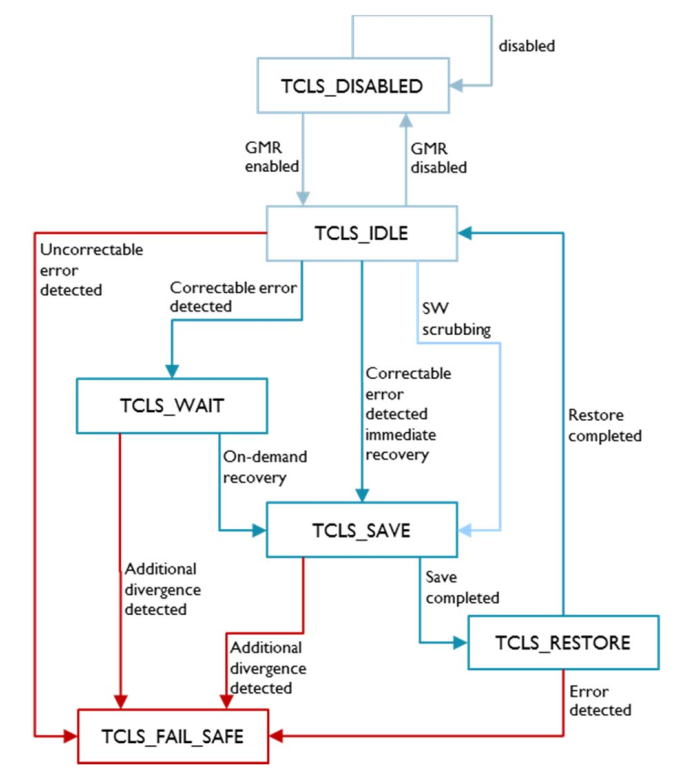
\includegraphics[width=0.9\linewidth]{images/tcls_resynchronization.png}
      \caption{TCLS resynchronization finite state machine \citep{TCLS_cortex_r}}
      \label{fig:tcls_resynchronization}
    
\end{figure}

\section{RAM error correction}

In microcontrollers, stray radiation and other effects can cause the data stored in RAM (random access memory) to be corrupted (bit flip).  The tightly coupled memories (TCMs) and caches on a Cortex-R processor can be configured to detect and correct errors that can occur in the RAMs. Extra, redundant data (checksum) is computed by the processor and stored in RAMs alongside the real data. When the processor reads the data from the RAM, it checks the redundant data matches the real data and can either signal an error, or attempt to correct the data.

Cortex-R5 allows the usage of:
\begin{itemize}

    \item parity,
    \item 64-bit ECC or
    \item 32-bit ECC \citep{cortex_r5_reference_manual}.
\end{itemize}

With parity, an error can be detected, but it can't be corrected. Using either 64-bit or 32-bit ECC (error checking and correction) detects up to two errors in a data chunk (either 64-bit or 32-bit) and correct any single error in the data chunk. Parity adds one redundant bit for every byte. 64-bit ECC adds one byte per 8-byte data chunk. 32-bit ECC adds seven bits per 4 bytes of the data chunk. 

Cortex-R8 uses 32-bit, 34-bit or 64-bit ECC of variable data chunks to protect its RAMs \citep{cortex_r8_reference_manual}.

\section{Interrupt handling}

According to \citep{cortex_r5_reference_manual}, Interrupt handling in the processor is compatible with previous ARM architectures, but has
several additional features to improve interrupt performance for real-time applications.

ARM Cortex-R5 connects the vectored interrupt controller (VIC) over a port, unlike ARM Cortex-M series microcontrollers that only have VIC close to the core. Having a VIC over the port provides faster interrupt entry, but one can disable it for compatibility with earlier interrupt controllers \citep{cortex_r5_reference_manual}. ARM Cortex-R5 doesn't allow tail chaining of the interrupts, nor the handling of late-arriving interrupts, unlike ARM Cortex-M series. 

Both ARM Cortex-R and Cortex-M series microcontrollers can abandon assembler instructions LDM and STM to lower the interrupt's latency. While Cortex-R microcontrollers will rerun the whole command upon the return from the interrupt, the ARM Cortex-M microcontrollers will just continue where they left of.

 

\section{CPU Compare Module for Cortex-R5F by Texas Instruments}

CPU compare module (CCM) detects run-time faults in devices like the CPU and VIM (vectored interrupt controller module) and forwards them to the next step in the error handling of the microcontroller i.e. to ESM (error signaling module). Alongside the run-time fault testing, CCM incorporates a self-test capability to allow for boot time checking of hardware faults within the CCM itself \citep{TMS570LS31x21x_manual}.

The main features of the CCM are:
\begin{itemize}

    \item{run-time detection of faults,}
    \item{self-test capability and}
    \item{error forcing capability.}

\end{itemize}

There are four modes of diagnostics for CPU/VIM output compare.
\begin{itemize}

    \item active compare lockstep,
    \item self-test,
    \item error forcing and
    \item self-test error forcing mode.

\end{itemize}

Active compare lockstep mode is defaulted to on start-up. The bus output signals of both CPU and VIMs are compared. List of all compared output signals is available in \citep[p. 500]{TMS570LS31x21x_manual}.

In self-test mode, test patterns are automatically generated by the CCM-R4F to
determine its correct functionality. In case of error detection that indicates a
hardware fault on the module itself, a “CCM-R4F - self-test” flag will be raised to
the ESM. After the completion or termination of the self-test, if no error occurred,
the self-test complete flag is set to notify the system to proceed appropriately. The compare match test and compare mismatch test are generated to ensure proper functioning. In compare match test an identical vector is applied to both input ports at the same time expecting a compare match. The compare mismatch test is similar to the compare match test, but one of the input vectors has one bit flipped. On the output, compare mismatch is expected.

Error forcing mode ensures that an error on the CCM's input is detected. In the case when the error from error forcing mode is not detected there is a hardware failure present. The difference between the compare mismatch test and error forcing mode is that error forcing mode ensures that compare error output signal asserts. This mode lasts for one CPU cycle.
